\begin{trapbox}
	\textbf{\textcolor{CTrap}{易错1｜把“最终更快”误记成“任何时候都更大”}}
	\textbf{错误想法：}$2^x$永远大于$x^2$。
	\textbf{反例：}当$x=3$时，$2^3=8<9=3^2$；当$x=5$时，$2^5=32>25=5^2$。中间发生过反超。
	\begin{center}
	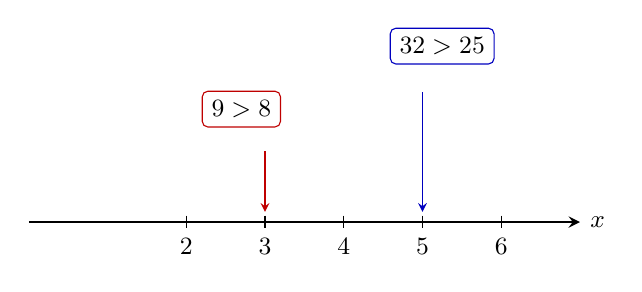
\begin{tikzpicture}[>=stealth,font=\small,x=1cm,y=1cm]
		\draw[->,thick] (0,0)--(7,0) node[right] {$x$};
		\foreach \x in {2,3,4,5,6} {\draw (\x,0.08)--(\x,-0.08) node[below]{\x};}
		\node[draw=red!75!black,rounded corners=2pt,above] at (2.7,1.2) {$9>8$};
		\node[draw=blue!75!black,rounded corners=2pt,above] at (5.25,2.0) {$32>25$};
		\draw[->,red!75!black] (3,0.9)--(3,0.13);
		\draw[->,blue!75!black] (5,1.65)--(5,0.13);
	\end{tikzpicture}

	\end{center}
	\textbf{正确理解：}结论说的是$x$足够大\textbf{以后}，不是某几个数，也不是全部$x$。

	\medskip
	\textbf{\textcolor{CTrap}{易错2｜忘记检查底数和指数}}
	\textbf{错误想法：}只要写成$a^x$，就一定比$x^\alpha$增长快。
	\textbf{反例：}$(\tfrac12)^x$随着$x$增大反而越来越小；$1^x$始终等于$1$；$x^0$也始终等于$1$。
	\begin{center}
	\begin{tikzpicture}[>=stealth,font=\small,x=1cm,y=1cm]
		\draw[->] (0,0)--(5.3,0) node[right] {$x$};
		\draw[->] (0,0)--(0,2.8) node[above] {$y$};
		\draw[red!75!black,very thick] plot[domain=0:5,samples=60] (\x,{pow(0.5,\x)});
		\draw[blue!75!black,very thick,dashed] (0,1)--(5,1);
		\node[anchor=west,red!75!black] at (1.1,2.25) {$(\frac12)^x$：越走越低};
		\node[anchor=west,blue!75!black] at (2.5,1.27) {$1^x=1$};
	\end{tikzpicture}

	\end{center}
	\textbf{正确理解：}本结论要求$a>1$、$\alpha>0$、$x\to+\infty$；三个条件缺一不可。

	\medskip
	\textbf{\textcolor{CTrap}{易错3｜比值写反，或加法里随手丢项}}
	\textbf{错误想法：}$\frac{x^{100}}{2^x}\to+\infty$，或者直接说$x^{10}+\log_3x=x^{10}$。
	\textbf{正确做法：}先判断谁更快，再看它在分子还是分母；\textbf{“相比起来很小”不等于“两者相等”}。
	\begin{center}
	\begin{tikzpicture}[>=stealth,font=\small]
		\node[draw=blue!65!black,rounded corners=3pt,inner sep=5pt] (a) at (0,0) {$\dfrac{2^x}{x^{100}}\to+\infty$};
		\node[draw=red!65!black,rounded corners=3pt,inner sep=5pt] (b) at (5.3,0) {$\dfrac{x^{100}}{2^x}\to0$};
		\draw[<->,thick] (a.east)--node[above] {倒过来} (b.west);
	\end{tikzpicture}

	\end{center}
	在例3中，应写成
	\[
		\frac{x^{10}+\log_3x}{4^x}
		=\frac{x^{10}}{4^x}\left(1+\frac{\log_3x}{x^{10}}\right),
	\]
	再判断两个部分的变化，不能把原式里的$\log_3x$当成真的$0$。
\end{trapbox}
